\chapter{Grundlagen}
    \section{Supervised Learning}
        \cite{supervised} Beim Supervised Learning gibt es sogenannte Features (Eingabedaten) \textbf{x}
        und Labels (Zielvariablen) \textbf{y}.
        Die Daten bestehen also aus Features und den dazugehörigen Labels.
        Ein Modell, welches diese Eingabedaten zum Trainieren erhält, versucht nun, einen Zusammenhang zwischen den Features und den Labels zu erkennen.
        Ein trainiertes Modell kann nun bei nicht gelabelten Eingabedaten das Label zu dem Datenpunkt, der dazugehört, vorhersagen.
        Supervised Learning zählt neben Unsupervised Learning und Reinforcement Learning zu einem der drei Teilaspekte, aus denen Machine Learning besteht.\\[2ex]
        Supervised Learning lässt sich unterteilen in zwei Arten:

        \begin{enumerate}
            \item Regression\\
                Zu einer Regression gehören alle Vorhersagen bei denen das Label kontinuierlich ist: $y \in \field{ R}$ \\
                Beispiele:
                \begin{itemize}
                    \item Vorhersage der Temperatur
                    \item Vorhersage des DAX
                    \item Vorhersage des Gewichts
                \end{itemize}
            \item Klassifizierung
                Vorhersagen bei denen das Label  Kategorisch ist, werden als Klassifizierung (Classification) bezeichnet.
                Es gibt zwei Arten von Klassifizierungen. Binäre Klassifizierung wenn es genau zwei Klassen gibt, sowie Mehrklassen-Klassifizierung.\\
                Beispiele:
                \begin{itemize}
                    \item 
                    \textbf{x}: Alle Pixel eines Bildes.\\
                    \textbf{y}: Welches Tier ist zu sehen? $y = 0$: "Katze", $y = 1$: "Hund", $y = 2$: "Maus" \\
                    $\rightarrow y \in \{0, 1, 2\}$
                    \item
                    \textbf{x}: Das Geschlecht einer Person \\
                    \textbf{y}: $y = 0$: Mann, $y = 1$: Frau \\
                    $\rightarrow y \in \{0, 1\}$
                \end{itemize}
        \end{enumerate}

\newpage
    \section{Unsupervised Learning} 
        \cite{unsupervised} Anders als beim Supervised Learning gibt es beim Unsupervised Learning keine Labels.
        Das Ziel besteht darin, innerhalb der Daten Strukturen und Muster zu erkennen.
        Es gibt verschiedene Arten des Unsupervised Learning.
        \begin{enumerate}
            \item Clustering
   
            Beim Clustering werden Datenpunkte in Gruppen unterteilt.
            Daten innerhalb einer Gruppe ähneln sich. Datenpunkte aus unterschiedlichen Gruppen weißen größere Unterschiede auf.
            \begin{figure}[!htb]
                \centering
                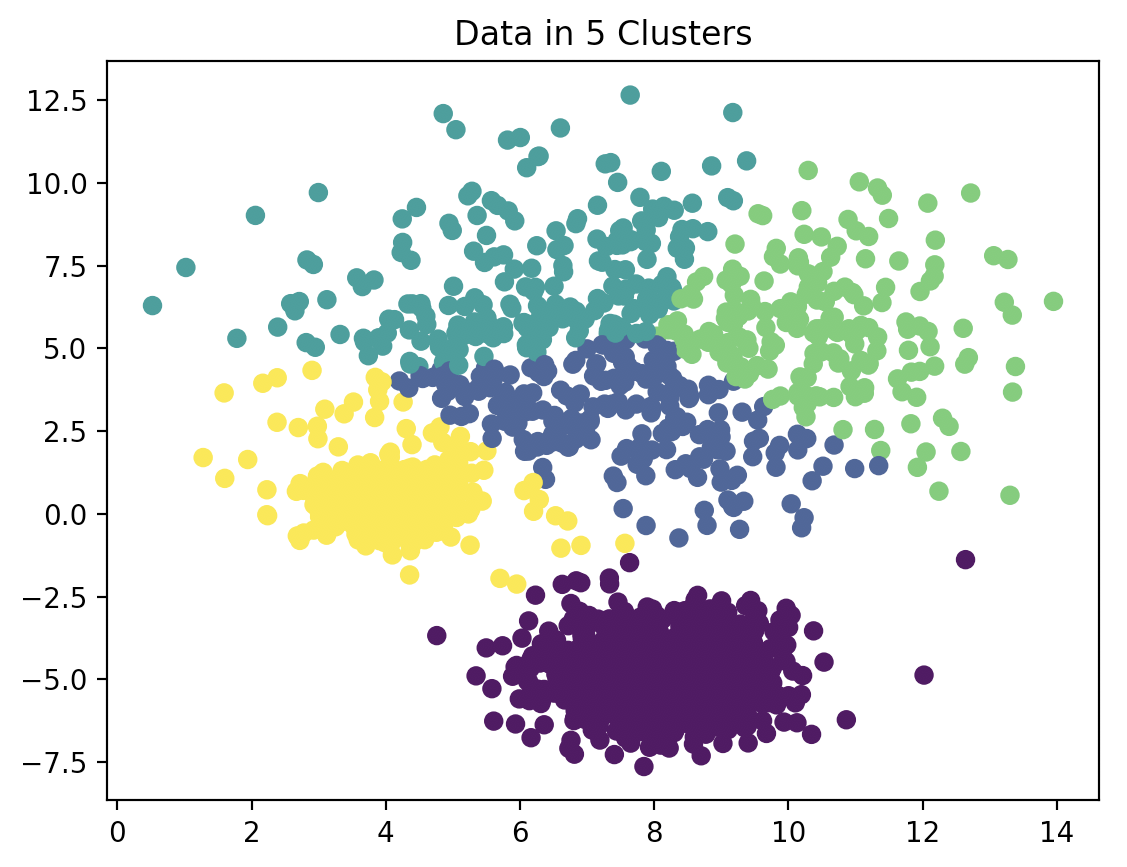
\includegraphics[scale=0.2]{pictures/k-means-clustering.png}
                \caption{Datenpunkte unterteilt in fünf Cluster \cite{k-means-clustering}.}
            \end{figure}
            \item Dimensionsreduktion

            Hierbei handelt es sich um Modelle, die Daten entgegennehmen und diese komprimieren.
            Dafür wird kein Label benötigt. Ein Beispiel ist ein Autoencoder, da dieser Daten komprimiert und anschließend wieder rekonstruiert. Hierfür werden lediglich die Features benötigt, jedoch keine Labels.
            Diese Art der Dimensionsreduktion wird im weiteren Verlauf dieses Kapitels genauer betrachtet.  
        \end{enumerate}

\newpage
    \section{Neural Networks}
        Ein neuronales Netz (Neural Network) ist eine Modellarchitektur,
        die aus sogenannten Neuronen und Schichten besteht.\\
        Es wird als „neuronales Netz“ bezeichnet, da es von den Gehirnen lebender Organismen inspiriert wurde.
        Gehirne besitzen ebenfalls Neuronen, die miteinander verbunden sind.
        Durch diese Verbindungen werden elektrische Signale geleitet, die das Denken ermöglichen.
        Ein neuronales Netz im Bereich der Informatik wird auch als künstliches neuronales Netz (KNN), englisch Artificial Neural Network (ANN), bezeichnet. Meist wird jedoch einfach die Abkürzung NN verwendet \cite{wikipedia_nn}.

        \subsection{Single-Layer Perceptrons}
            Die einfachste Form eines neuronalen Netzes ist ein einfaches Perzeptron (Single-Layer Perceptron). Es besteht aus zwei Schichten: der Eingabeschicht (Inputlayer), die für jeden Eingabepunkt ein Neuron enthält, und der Ausgabeschicht (Outputlayer), die aus einem Neuron für jede Ausgabe-Klasse besteht.
            Diese Art von Modellarchitektur gehört zum Supervised Learning.
            
            Single-Layer Perceptrons sind jedoch nur für sehr einfache Aufgaben geeignet,
            beispielsweise das Lernen einer logischen ODER- oder UND-Funktion.
            Single-Layer Perceptrons implementieren eine Binärklassifizierung, da es nur zwei Output-Neuronen gibt, 
            wie in Abbildung 1 zu sehen ist \cite{perceptrons}.
        
            \begin{figure}[!htb]
                \centering
                \includegraphics[width=11cm]{pictures/NN.pdf}
                \caption{Hier ist ein Single-Layer Perceptron zu sehen.}
            \end{figure}
        

\newpage
        \subsection{Deep Neural Networks}
            Tiefe neuronale Netze, im Englischen Deep Neural Networks (DNN), unterscheiden sich von Single-Layer Perceptrons darin, dass sie nicht nur eine Eingabeschicht und eine Ausgabeschicht besitzen, sondern auch versteckte Schichten (Hidden Layers) enthalten.
            Alle versteckten Schichten befinden sich zwischen der Eingabe- und der Ausgabeschicht.
            Ein DNN kann beliebig viele versteckte Schichten haben. Die Anzahl ist frei wählbar, es muss jedoch mindestens eine versteckte Schicht vorhanden sein, damit es als DNN gezählt wird.
            Die Anzahl der Neuronen in solchen versteckten Schichten kann ebenfalls beliebig variieren und ist somit ebenfalls frei wählbar.
            Je nach Design gibt es DNNs in den verschiedensten Größen und Komplexitätsstufen.
            Da die meisten neuronalen Netze versteckte Schichten besitzen, handelt es sich fast immer um DNN. Deshalb wird in der Regel einfach von neuronalen Netzen gesprochen, auch wenn DNNs gemeint sind. \newline
            \begin{figure}[!htb]
                \centering
                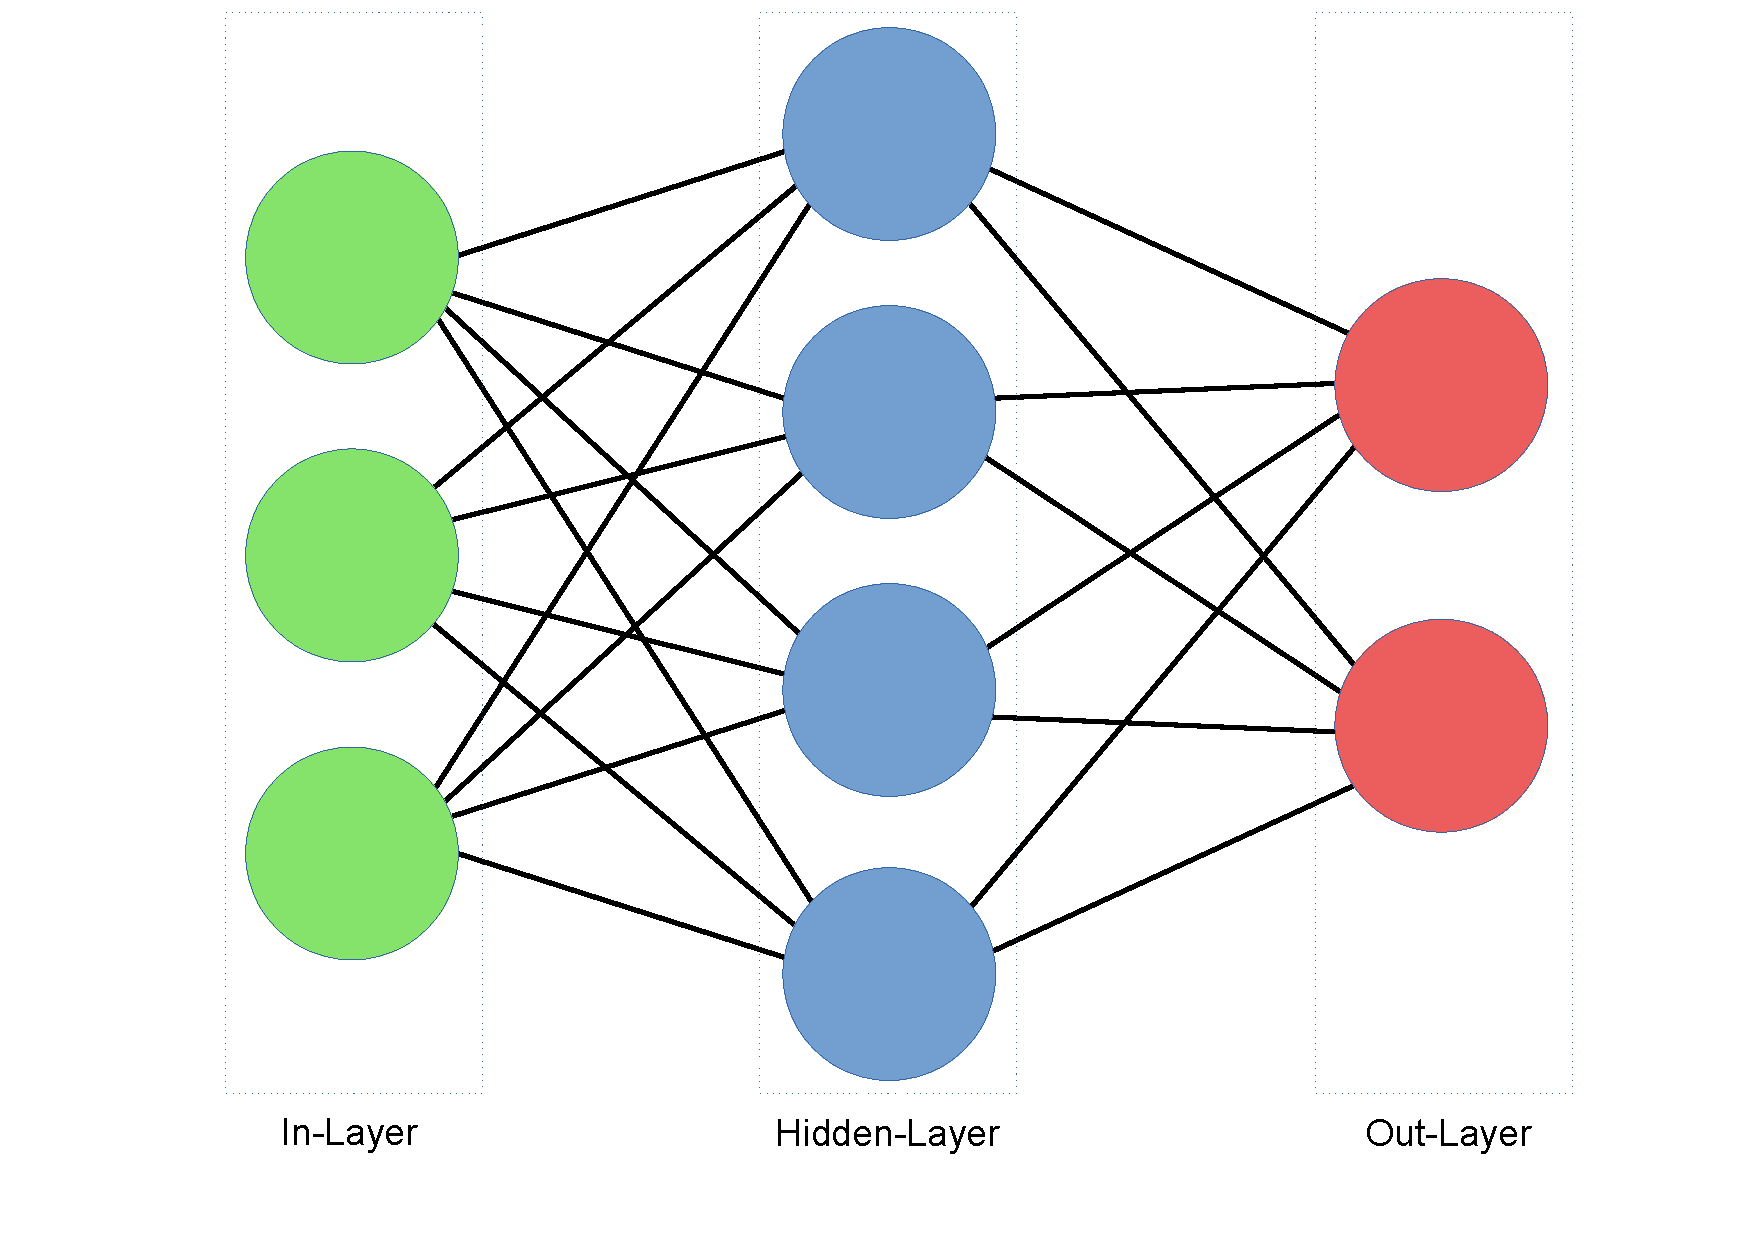
\includegraphics[width=11cm]{pictures/DNN.pdf}
                \caption{Hier ist ein Deep Neural Network mit einer versteckten Schicht zu sehen.}
            \end{figure}

\newpage
        \subsection{Convolutuional Neural Networks}
            \cite{convolutional} Convolutional Neural Networks (CNN) sind eine spezielle Architektur von
            künstlichen neuronalen Netzen, die besonders für die Verarbeitung von Daten mit räumlicher Struktur, wie z.B. Bildern, geeignet sind. Sie zeichnen sich durch den Einsatz von Faltungsschichten (Convolutional Layers) aus, die lokale Merkmale in den Eingabedaten extrahieren.
            Eine typische CNN-Architektur besteht aus drei Hauptkomponenten:

            \begin{enumerate}
                \item Convolutional Layers:\\
                    Diese Schichten führen die Faltung durch und erzeugen Feature Maps, die charakteristische Muster wie Kanten, Texturen oder Formen erkennen.
                \item Pooling Layers:\\
                    Diese Schichten reduzieren die räumliche Größe der Feature Maps und verringern so die Anzahl der Parameter, was die Berechnung effizienter macht und die Generalisierungsfähigkeit erhöht.
                \item Fully Connected Layers:\\
                    In diesen Schichten werden die extrahierten Merkmale für die Klassifikation oder andere Aufgaben genutzt.
            \end{enumerate} 
            
            CNNs sind bekannt für ihre Effektivität bei Aufgaben wie Bildklassifikation, Objekterkennung und Bildsegmentierung. Zu den erfolgreichsten Architekturen zählen Modelle wie AlexNet, VGG und ResNet, die sich durch fortschrittliche Designprinzipien und leistungsstarke Ergebnisse auszeichnen.

            Dank ihrer Fähigkeit, automatisch relevante Merkmale aus Rohdaten zu extrahieren, haben CNNs die Entwicklung in Bereichen wie Computer Vision, autonomes Fahren und medizinische Bildverarbeitung revolutioniert.

            \begin{figure}[!htb]
                \centering
                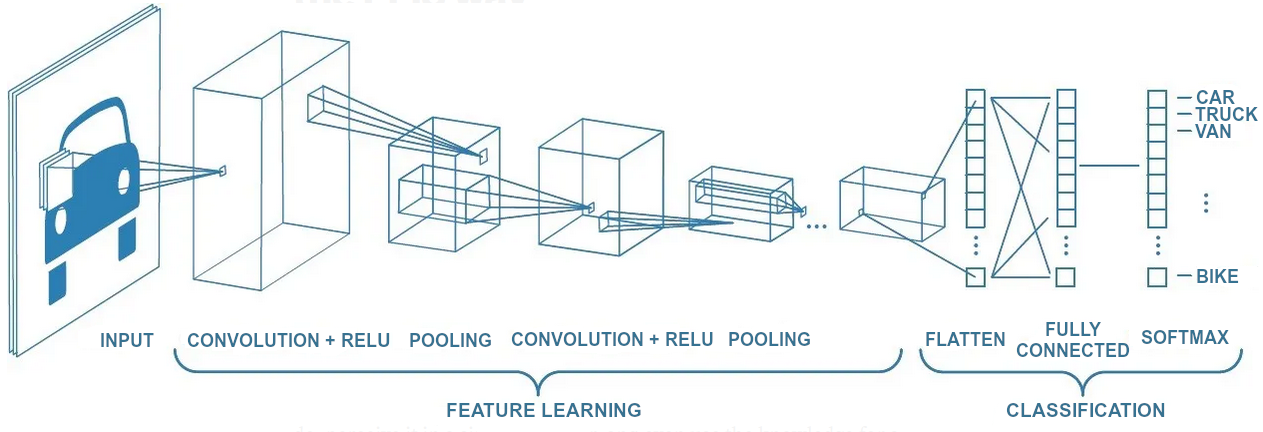
\includegraphics[scale=0.42]{pictures/cnn_auto.png}
                \caption{Visualisierung eines CNN \cite{cnn_auto}.}
            \end{figure}
            
\newpage
    \section{Kompression von Bildern}
        \subsection{Traditionelle Bildkompression}
            \cite{jpeg_paper, wikipedia_jpeg} JPEG wurde 1992 von der Joint Photographic Experts Group, einer internationalen Organisation für Bildstandards, eingeführt.\\
            JPEG-Dateien unterstützen eine Farbtiefe von bis zu 24 Bit und gehören zu den verlustbehafteten Komprimierungsverfahren für Bilder. Das bedeutet, dass bei der Reduzierung der Dateigröße zugunsten des Speicherplatzes Qualitätsverluste in Kauf genommen werden. Wie stark die Komprimierung erfolgen soll und damit auch der Qualitätsverlust, bleibt dem Nutzer überlassen.
            Dies wird durch die sogenannte Kompressionsqualität beschrieben, die als prozentualer Wert angegeben wird. Eine Kompressionsqualität von 100 entspricht nahezu verlustfreier Speicherung, während eine niedrigere Qualität zu stärkeren Verlusten führt – jedoch zugunsten einer kleineren Dateigröße.

            \begin{enumerate}
                \item Vorteile
                \begin{itemize}
                    \item Hohe Kompression von Bildern.
                    \item Flexible Anpassung der Qualität des Benutzers je nach Bedarf.
                    \item Das JPEG-Format wird so gut wie von allen Geräten und Software unterstützt.
                    \item Effiziente Speicherung und Übertragung,\\
                    da sie klein sind was den Speicherbedarf anbelangt.
                \end{itemize}
                \item Nachteile
                \begin{itemize}
                    \item Verlustbehaftete Kompression führt immer zu Qualitätsverlust.
                    \item Hohe Kompressionen erzeugen sichtbare Artefakte.
                    \item JPEG unterstützt keine Transparenz wie das PNG-Format.
                    \item JPEG unterstützt lediglich $8$-Bit Farbtiefe pro Farbkanal.
                \end{itemize}
            \end{enumerate} 

            JPEG eignet sich somit hervorragend für Bilder, wenn man Qualitätsverluste zugunsten eines geringeren Speicherbedarfs tolerieren kann.

\newpage
        \subsection{Autoencoder}
            Ein Autoencoder ist ein neuronales Netzwerk, das aus zwei Hauptkomponenten besteht: einem Encoder und einem Decoder. Der Encoder komprimiert die Eingabedaten, indem er die relevantesten Merkmale extrahiert und diese in eine kleiner dimensionierte Darstellung überführt, die als latenter Raum oder „Code“ bezeichnet wird. Der Decoder rekonstruiert aus dieser komprimierten Darstellung die ursprünglichen Daten \cite{covalent_ae, ae_paper}.

            Autoencoder werden zur Dimensionsreduktion und Datenkompression eingesetzt. Sie lernen effiziente Einbettungen von nicht gelabelten Daten und sorgen dafür, dass der latente Raum die wesentlichen Informationen des Datensatzes enthält. Das Ziel des Decoders ist es, die Ausgangsdaten möglichst genau wiederherzustellen, wodurch sichergestellt wird, dass der latente Raum die wichtigsten Informationen des Datensatzes repräsentiert \cite{towards_ae_vae}.
            Autoencoder haben die klassischen technischen Verfahren in Bezug auf Genauigkeit und Leistung bei einer Vielzahl von Anwendungen übertroffen, z.B. bei der Anomalieerkennung, Texterzeugung, Bilderzeugung, Bildentrauschung und der digitalen Kommunikation \cite{math_works}.


            \begin{figure}[!htb]
                \centering
                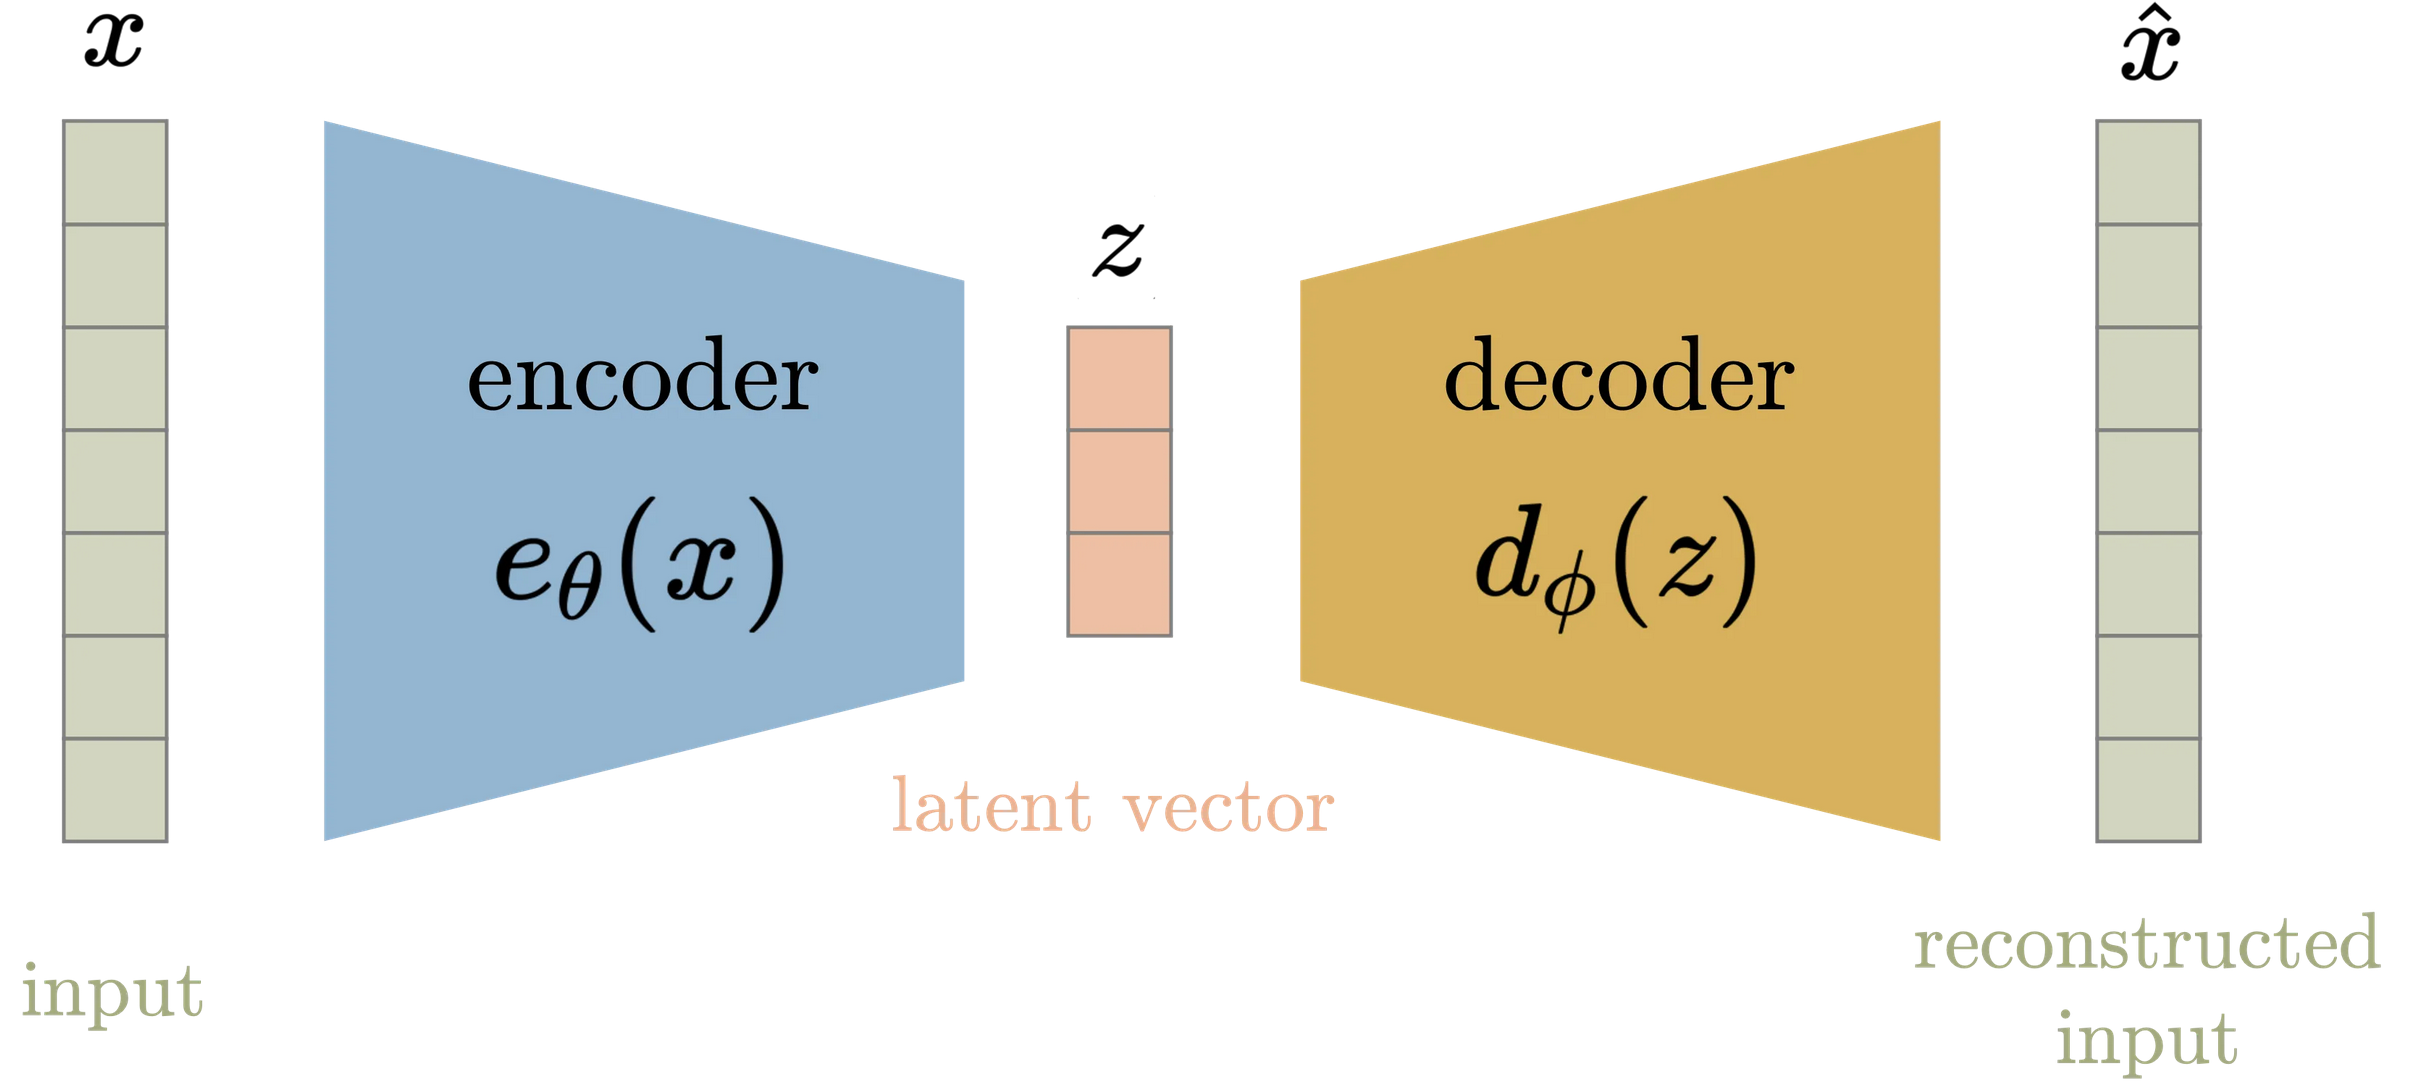
\includegraphics[scale=0.20]{pictures/ae.png}
                \caption{Skizze eines Autoencoders \cite{towards_ae_vae}.}
            \end{figure}

\newpage
            Der Autoencoder lernt die Funktion
            $e_{\theta}: \mathbb{R}^n \rightarrow \mathbb{R}^p \, \text{(Encoder)}$ und \\
            $d_{\phi} : \mathbb{R}^p \rightarrow \mathbb{R}^n \, \text{(Decoder)}$
            welche folgende Bedingung erfüllen muss.\bigskip
            \begin{center}
                $\argmin_{e_{\theta},d_{\phi}} \, \mathbb{E} \left[ \Delta \left( x, d_{\phi}(e_{\theta}(x)) \right) \right]$ \\
            \end{center}
   
            wobei $\mathbb{E}$ den Erwartungswert über die Verteilung von $x$ darstellt und $\Delta$ die Funktion für den Rekonstruktionsverlust ist,
            die die Distanz zwischen der Ausgabe des Decoders und der Eingabe misst \\
            (\emph{Dor Bank, Noam Koenigstein, Raja Giryes}, 3. Apr 2021, Paper zu Autoencoders). \\
            Anders ausgedrückt ist der Loss:
            \begin{center}
                $L(\theta, \phi) = ||x - \hat{x}||_{2}^2 = ||x - d_{\phi}(z)||_{2}^2 = ||x - d_{\phi}(e_{\theta}(x))||_{2}^2$
            \end{center}

            Während des Trainings werden die Eingabedaten $x$ in den Encoder $e_{\theta}(x)$ hineingegeben.
            Diese Funktion enkodiert die Daten durch mehrere Schichten in eine kleinere latente Dimension $z$.
            Anschließend wird $z$ dem Decoder übergeben, dessen Funktion den latenten Vektor zurück in ein $\hat{x}$ dekodiert.
            Das Modell wird mithilfe einer Verlustfunktion trainiert, die dafür sorgt, dass der sogenannte Mean Squared Error (MSE) zwischen $x$ und $\hat{x}$ so gering wie möglich wird \cite{towards_ae_vae, ae_paper}.

            \begin{figure}[!htb]
                \centering
                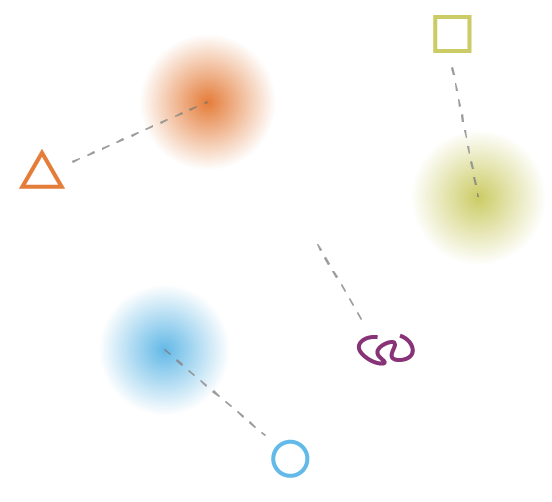
\includegraphics[scale=0.38]{pictures/Autoencoder_Latentdim.png}
                \caption{Latenter Raum eines AE \cite{towards_ae_vae, uni_hamburg}.}
            \end{figure}

            Das Problem eines Autoencoders ist, dass er lediglich die Daten komprimiert, jedoch der latente Raum eine deterministische Repräsentation liefert. Das bedeutet, dass alle Eingaben auf einen festen Punkt im latenten Raum abgebildet werden.
            Es wird keine Wahrscheinlichkeitsverteilung berücksichtigt.
            Dadurch gibt es keine Zusammenhänge zwischen ähnlichen Datenpunkten im latenten Raum.
            Der Autoencoder ist somit nicht in der Lage, neue brauchbare Daten zu generieren, sondern lediglich Eingabedaten zu rekonstruieren \cite{py_mage}.
            
\begin{comment}            
\newpage
 
\textbf{Autoencoder (AE)}
\begin{minted}[linenos, fontsize=\footnotesize, frame=lines]{python}
class Encoder(nn.Module):
    def __init__(self, width, height, latent_dim):
        super(Encoder, self).__init__()
        
        self.encoder = nn.Sequential(
            nn.Linear(height*width, 1024),
            nn.ReLU(True),
            nn.Linear(1024, 128),
            nn.ReLU(True),
            nn.Linear(128, 64),
            nn.ReLU(True),
            nn.Linear(64, latent_dim),
            nn.ReLU(True)
        )

    def forward(self, x):
        out = self.encoder(x) 
        return out

class Decoder(nn.Module):
    def __init__(self, width, height, latent_dim):
        super(Decoder, self).__init__()
        
        self.decoder = nn.Sequential(
            nn.Linear(latent_dim, 64),
            nn.ReLU(True),
            nn.Linear(64, 128),
            nn.ReLU(True),
            nn.Linear(128, 1024),
            nn.ReLU(True),
            nn.Linear(1024, height*width),
            nn.Sigmoid()
        )
        
    def forward(self, x):
        out = self.decoder(x)       
        return out

class Autoencoder(nn.Module):
    def __init__(self, width, height, latent_dim):
        super(Autoencoder, self).__init__()
        self.width = width
        self.height = height
        self.latent_dim = latent_dim
        self.encoder = Encoder(width, height, latent_dim)
        self.decoder = Decoder(width, height, latent_dim)

    def forward(self, x):   
        x = x.view(x.size(0), -1)
        out = self.encoder(x) 
        out = self.decoder(out)
        out = out.view(out.size(0), -1, self.width, self.height)  
        return out
\end{minted}

\textbf{Covolutional Autoencoder (CAE)}
\begin{minted}[linenos, fontsize=\footnotesize, frame=lines]{python}
class Encoder(nn.Module):
    def __init__(self, in_channels, latent_dim):
        super(Encoder, self).__init__()
        
        self.encoder = nn.Sequential(
            nn.Conv2d(in_channels, 1024, kernel_size=4, stride=2, padding=1),
            nn.ReLU(True),
            nn.Conv2d(1024, 128, kernel_size=4, stride=2, padding=0),
            nn.ReLU(True),
            nn.Conv2d(128, 64, kernel_size=4, stride=2, padding=1),
            nn.ReLU(True),
            nn.Conv2d(64, latent_dim, kernel_size=3, stride=1, padding=0),
            nn.ReLU(True)
        )

    def forward(self, x):
        out = self.encoder(x)    
        return out

class Decoder(nn.Module):
    def __init__(self, out_channels, latent_dim):
        super(Decoder, self).__init__()
        
        self.decoder = nn.Sequential(
            nn.ConvTranspose2d(latent_dim, 64, kernel_size=3, stride=1,
            padding=0),
            nn.ReLU(True),
            nn.ConvTranspose2d(64, 128, kernel_size=4, stride=2, padding=1),
            nn.ReLU(True),
            nn.ConvTranspose2d(128, 1024, kernel_size=4, stride=2, padding=0),
            nn.ReLU(True),
            nn.ConvTranspose2d(1024, out_channels, kernel_size=4, stride=2,
            padding=1),
            nn.Sigmoid()
        )
        
    def forward(self, x):
        out = self.decoder(x)    
        return out

class Conv_Autoencoder(nn.Module):
    def __init__(self, in_channels, out_channels, latent_dim):
        super(Conv_Autoencoder, self).__init__()
        
        self.encoder = Encoder(in_channels, latent_dim)
        self.decoder = Decoder(out_channels, latent_dim)

    def forward(self, x):
        out = self.encoder(x)        
        out = self.decoder(out)
        return out
\end{minted}
            Der Quelltext in PyTorch für zwei Autoencoder:
            Der Vorteil eines Convolutional Autoencoders (CAE) gegenüber eines Autoencoders (AE) mit linearen Schichten (Fully Connected Layers) ist, dass er bessere Ergebnisse bei der Bildverarbeitung liefert, dank seiner Convolutional Schichten.
            Ein weiterer Vorteil ist, dass er Bilder unabhängig von ihrer Größe $H \times W$ entgegennehmen kann.
            Dies ermöglicht es einem Autoencoder, der nur aus Convolutional Schichten besteht, jede beliebige Bildgröße zu verarbeiten.
\end{comment}
    
\newpage
        \subsection{Variational Autoencoder}   
            \cite{towards_ae_vae, py_mage} Wie ein Autoencoder besteht auch ein Variational Autoencoder (VAE) aus zwei Teilen:
            Einem Encoder-Teil, der den Input entgegennimmt und diesen in den latenten Raum enkodiert, sowie einem Decoder-Teil, der aus dem latenten Raum versucht, das Original wieder zu rekonstruieren.
            Allerdings erweitern VAEs die Idee von Autoencodern. Denn ein VAE lernt keine deterministischen Werte, sondern eine Verteilung der Daten. Anders als beim AE ist der latente Raum keine deterministische Repräsentation der Daten, sondern eine probabilistische Interpretation, da eine Wahrscheinlichkeitsverteilung über diesen Raum gelernt wird.
            Die Idee ist also, dass Daten im latenten Raum nicht als einzelner Punkt $z$ dargestellt werden, sondern als eine Wahrscheinlichkeitsverteilung $p(z)$.
            So lernt der VAE für die latenten Variablen eine Verteilung \cite{vae_paper_1, vae_paper_2}.
            
            Das Ziel dieser probabilistischen Interpretation ist, dass nun ähnliche Eingabedaten im Latentenraum an ähnlichen oder naheliegenden Bereichen liegen.
            Dies führt zu einer besseren Generalisierung und ermöglicht es nun nicht nur, Daten zu rekonstruieren, sondern auch, neue Daten zu generieren.

            \begin{figure}[!htb]
                \centering
                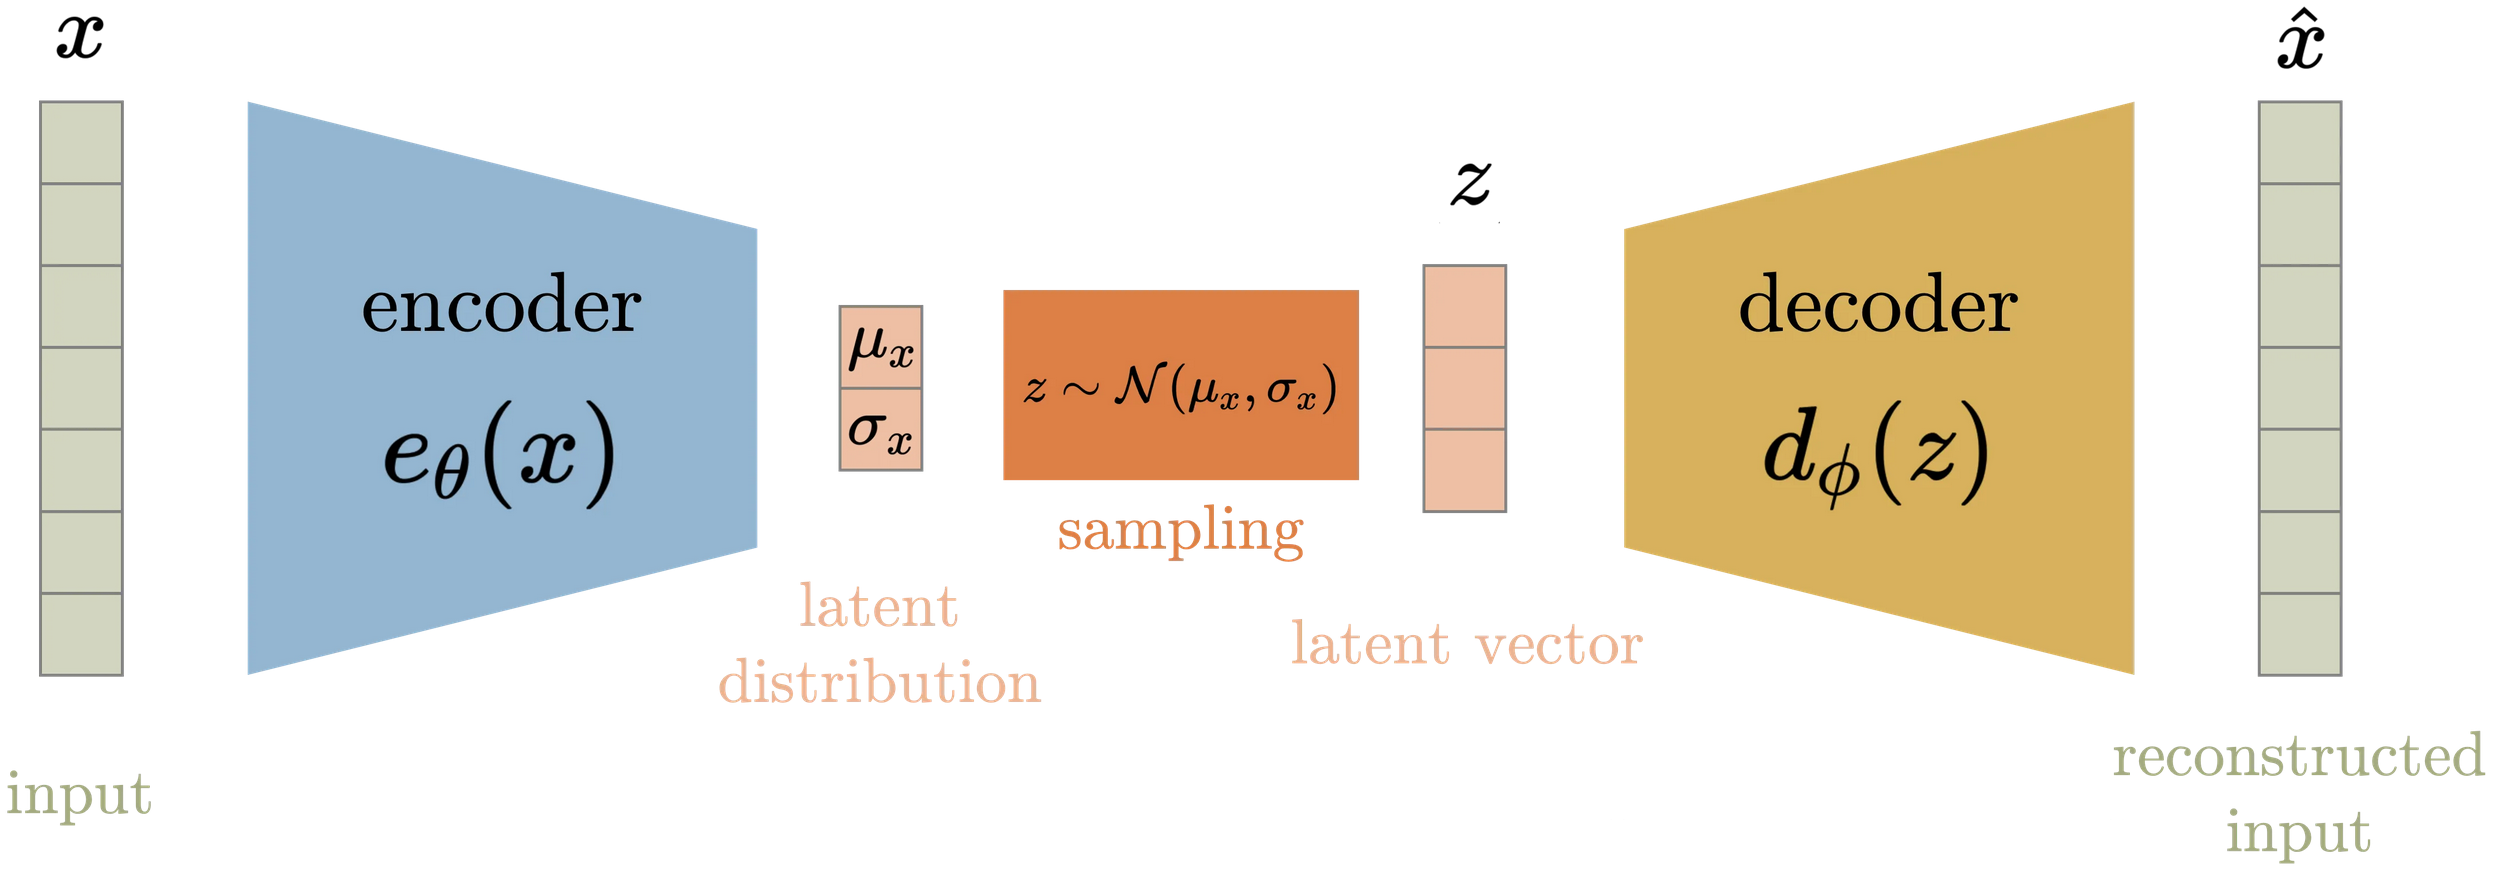
\includegraphics[scale=0.22]{pictures/vae.png}
                \caption{Skizze eines Variational Autoencoders \cite{towards_ae_vae}.}
            \end{figure}

            Ein VAE lernt also die Funktion
            $e_{\theta}: \mathbb{R}^n \rightarrow \mathbb{R}^p \, \text{(Encoder)}$ und \\
            $d_{\phi} : \mathbb{R}^p \rightarrow \mathbb{R}^n \, \text{(Decoder)}$,
            unter der Annahme, dass \bigskip

            \begin{center}
                $(\mu_{\theta}(x), \sigma_{\theta}(x)) = e_{\theta}(x)$ und $\hat{x} = d_{\phi}(z)$,\vspace{1mm}\\
                $q_\theta(z \mid x) = N(z | \mu_\theta(x), \sigma_\theta^2(x) I)$ und
                $p_\phi(\hat{x} \mid z) = N\left(\hat{x} | \mu_\phi(z), \sigma_\phi^2(z) I\right)$,\vspace{1mm}\\
                $z \sim q_\theta(z \mid x)$ und $\hat{x} \sim p_\phi(\hat{x} \mid z)$ sowie\vspace{1mm}\\
                $p(z) = N(0, I)$ und\vspace{1mm}\\
                $\argmin_{e_\theta, d_\phi} \left( \mathbb{E}[ \Delta(x, d_\phi(e_\theta(x))) ] +
                D_{KL}(q_\theta(z \mid x) \| p(z)) \right)$
            \end{center}
\newpage
            Diese Formel beschreibt die Optimierungsaufgabe eines Variational Autoencoders (VAE).
            Sie zeigt, wie die Parameter $\theta$ des Encoders sowie $\phi$ des Decoders angepasst werden, damit das Modell möglichst verlustfreie Vorhersagen treffen kann.
    
            Der VAE hat zwei Verlustfunktionen. Der Reconstruction Loss misst, wie stark sich die rekonstruierte Ausgabe von der Eingabe unterscheidet. Des Weiteren gibt es die KL-Divergenz (Kullback-Leibler-Divergenz), die den Unterschied zwischen der latenten Verteilung $q_\theta(z \mid x)$ und der gewünschten Verteilung $p(z)$, also der Normalverteilung, misst. Das Ziel ist es, den regularisierten Raum so nah wie möglich an die Normalverteilung zu bringen \cite{towards_ae_vae, vae_paper_1, vae_paper_2}.\bigskip
            \begin{center}
                $reconstruction \ loss = \| x - d_\phi(\mu_\theta(x) + \sigma_\theta(x) \cdot \epsilon) \|_2^2$\vspace{1mm}\\
                $KL-Divergenz = D_{KL}(q_\theta(z \mid x) \| p(z))$\vspace{1mm}\\
                $L(\theta, \phi) = \| x - d_\phi(\mu_\theta(x) + \sigma_\theta(x) \cdot \epsilon) \|_2^2 +
                D_{KL}(q_\theta(z \mid x) \| p(z))$
            \end{center}
            \bigskip

            Die folgenden Schritte zeigen den Ablauf eines VAE:
            \begin{enumerate}
                \item Input\\
                    Der Encoder nimmt die Eingabedaten entgegen, die kodiert werden sollen.
                \item Mittelwert und Standartabweichung\\
                    Der Encoder erzeugt eine latente Distribution bestehend aus Standartabweichung $\sigma$ und Mittelwert $\mu$.
                \item Sampling\\
                    Um $z$ zu berechnen wird ein zufälliger Datenpunkt $\epsilon$ aus der Normalverteilung $q_\theta(z \mid x)$ gewählt.\\
                    $z = \mu_\theta(x) + \sigma_\theta(x) \cdot \epsilon$
                \item Rekonstruktion\\
                    $z$ wird dann dem Decoder übergeben welcher lernt aus der Wahrscheinlichkeitsverteilung das Bild erneut zu Rekonstruieren. 
            \end{enumerate}
\newpage   
            Da im Gegensatz zu einem AE der latente Raum nun auf einer Normalverteilung beruht, sind bei einem VAE ähnliche Daten in Clustern zusammengefasst. Dies ermöglicht es, mit einem VAE sinnvolle Daten zu generieren.
    
            \begin{figure}[!htb]
                \centering
                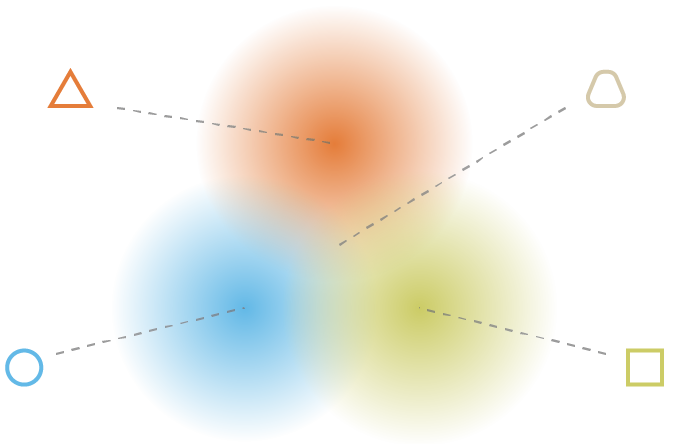
\includegraphics[scale=0.35]{pictures/VAE_Latentdim.png}
                \caption{Latenter Raum eines VAE \cite{towards_ae_vae, uni_hamburg}.}
            \end{figure}

            \begin{figure}[!htb]
                \centering
                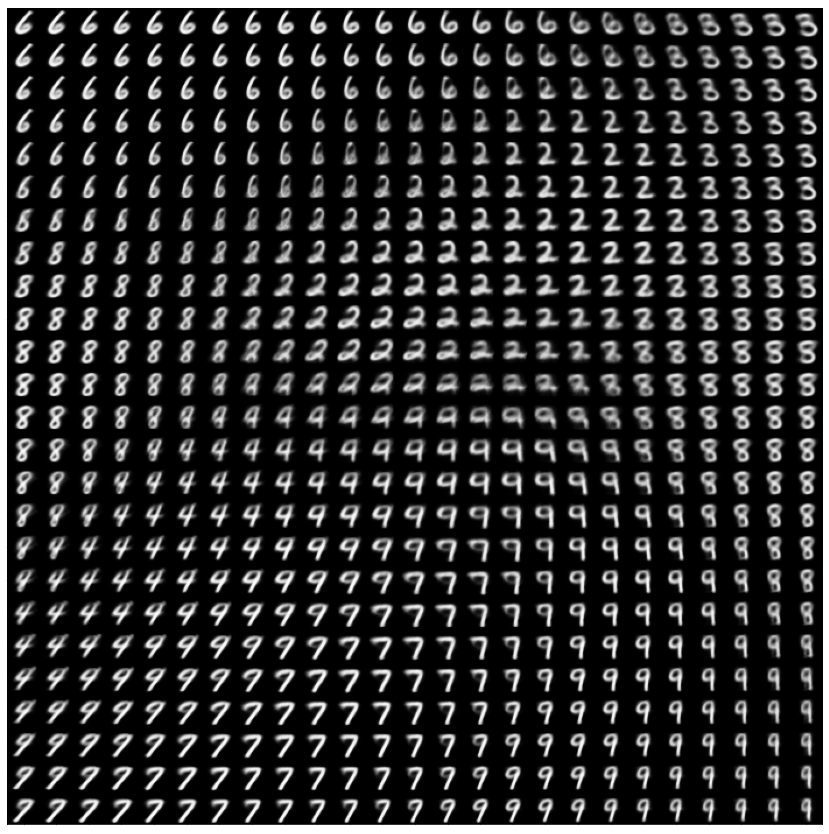
\includegraphics[scale=0.32]{pictures/mnist latent dim.png}
                \caption{Latenter Raum eines VAE dargestellt mit dem MNIST-Datensatz \cite{vae_keras}.}
            \end{figure}

\begin{comment}
\newpage
\textbf{Variational Autoencoder (VAE)}
\begin{minted}[linenos, fontsize=\footnotesize, frame=lines]{python}
class Encoder(nn.Module):
    def __init__(self, in_channels, latent_dim):
        super(Encoder, self).__init__()
        
        self.encoder = nn.Sequential(
            nn.Conv2d(in_channels, 1024, kernel_size=4, stride=2, padding=1),
            nn.ReLU(True),
            nn.Conv2d(1024, 128, kernel_size=4, stride=2, padding=0),
            nn.ReLU(True),
            nn.Conv2d(128, 64, kernel_size=4, stride=2, padding=1),
            nn.ReLU(True)
        )

        self.conv_mu = nn.Conv2d(64, latent_dim, kernel_size=3, stride=1, padding=0)
        self.conv_logvar = nn.Conv2d(64, latent_dim, kernel_size=3, stride=1, padding=0)

    def forward(self, x):
        out = self.encoder(x)
        mu = self.conv_mu(out)
        logvar = self.conv_logvar(out)
        return mu, logvar

class Decoder(nn.Module):
    def __init__(self, out_channels, latent_dim):
        super(Decoder, self).__init__()
        
        self.decoder = nn.Sequential(
            nn.ConvTranspose2d(latent_dim, 64, kernel_size=3, stride=1, padding=0),
            nn.ReLU(True),
            nn.ConvTranspose2d(64, 128, kernel_size=4, stride=2, padding=1),
            nn.ReLU(True),
            nn.ConvTranspose2d(128, 1024, kernel_size=4, stride=2, padding=0),
            nn.ReLU(True),
            nn.ConvTranspose2d(1024, out_channels, kernel_size=4, stride=2, padding=1),
            nn.Sigmoid()
        )
        
    def forward(self, x):
        out = self.decoder(x)    
        return out

class VAE(nn.Module):
    def __init__(self, in_channels, out_channels, latent_dim):
        super(VAE, self).__init__()
        
        self.encoder = Encoder(in_channels, latent_dim)
        self.decoder = Decoder(out_channels, latent_dim)

    def reparameterize(self, mu, logvar):
        std = torch.exp(0.5 * logvar)
        eps = torch.randn_like(std).to(DEVICE)
        return mu + eps * std

    def forward(self, x):
        mu, logvar = self.encoder(x)
        z = self.reparameterize(mu, logvar)
        x_hat = self.decoder(z)
        return x_hat, mu, logvar
\end{minted}
\end{comment}

\newpage
        \subsection{Vector Quantized Variational Autoencoder}
            \begin{figure}[!htb]
                \centering
                \includegraphics[scale=0.5]{pictures/catdog.png}
                \caption{Comic Figur Catdog aus der Serie Catdog \cite{catdog, cat, dog}.}
            \end{figure}
    
            Wie in \cite{vqvae_paper, vqvae_super, vqvae} beschrieben, ist ein Vektor Quantized Variational Autoencoder (VQ-VAE) eine Erweiterung des klassischen VAE. Während ein VAE die Daten in eine stetige Repräsentation des latenten Raums überführt, wird bei einem VQ-VAE die latente Repräsentation der Daten diskret. Die Motivation hinter dieser Diskretisierung liegt darin, dass wir in einer diskreten Welt leben. Es gibt keine Zwischenzustände wie „halb Mensch, halb Baum“ oder „halb Hund, halb Katze“. Ein VQ-VAE zielt darauf ab, die Daten auf eine diskrete Weise zu quantisieren.

            Wie alle anderen Autoencoder-Modelle besteht auch ein VQ-VAE aus einem Encoder und einem Decoder. In der Mitte befindet sich zusätzlich ein Quantifizierer und ein sogenanntes Codebook. Das Codebook ist eine Lookup-Tabelle, in der sogenannte Embedding-Vektoren gespeichert sind.
            Der Encoder kodiert die Eingabedaten zu einem latenten Vektor der Dimension $D$, der einen Datenpunkt im latenten Raum repräsentiert. Im Quantifizierungsschritt wird im Codebook nach dem nächstliegenden Embedding-Vektor (Codebook-Vektor)  gesucht und ersetzt den latenten Vektor durch diesen. Anschließend wird der neue latente Vektor, welcher ersetzt wurde, durch den Decoder wieder rekonstruiert.
            Die Embedding-Vektoren im Codebook müssen dabei die gleiche Dimension $D$ wie der latente Vektor haben.
    
\newpage
            \begin{figure}[!htb]
                \centering
                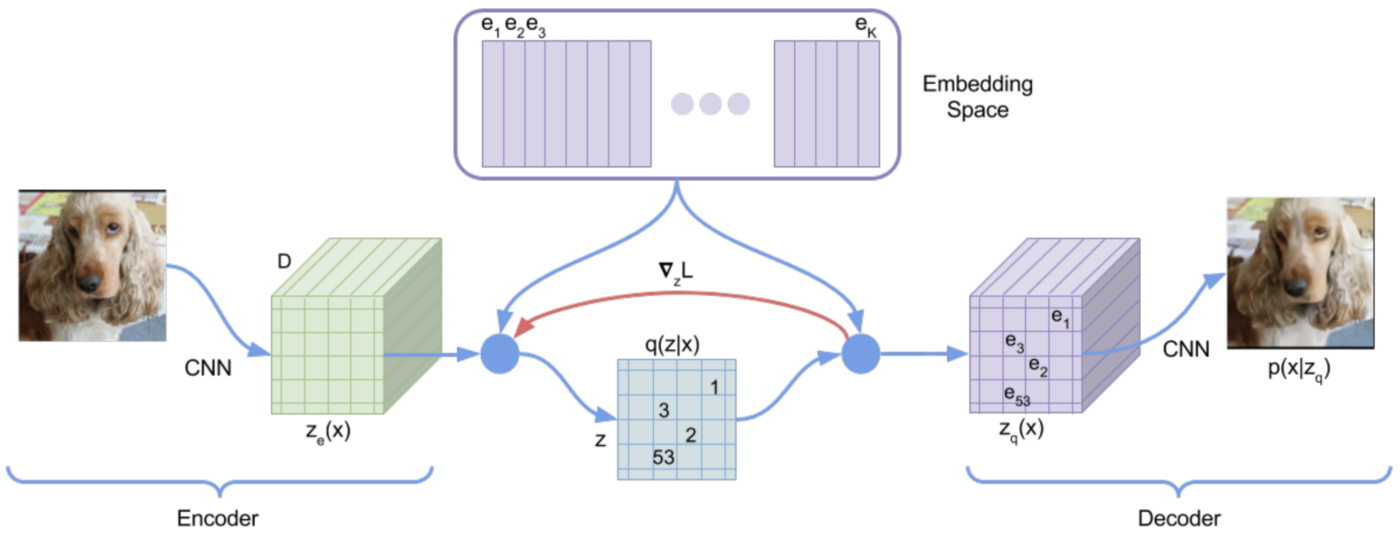
\includegraphics[scale=0.29]{pictures/vq-vae.png}
                \caption{Architektur eines VQ-VAE mit Straight-through estimation \cite{vqvae_pic}.}
            \end{figure}

            Ein VQ-VAE lernt die Funktion\\
            $e_{\theta}: \mathbb{R}^n \rightarrow \mathbb{R}^D_z \, \text{(Encoder)}$,
            $\mathbb{R}^D_z \rightarrow \mathbb{R}^D_q \text{(Quantifizierer)}$ und
            $d_{\phi} : \mathbb{R}^D_q \rightarrow \mathbb{R}^n \, \text{(Decoder)}$.
            \bigskip

            \begin{center}
                Der latente Raum ist definiert als $z_e(x) = e_\theta(x)$.\\
                Der Embedding-Space ist definiert als $e \in \mathbb{R}^{K \times D}$. \\
                $e_i \in \mathbb{R}^D, \; i \in \{1, 2, \dots, K\}$\\
                $K = Anzahl \ Codebook \ Vektoren$ und\\
                $D = Dimension \ jedes \ Latenten \ und \ Embedding \ Vektors$.\\
            \end{center}
            \begin{center}
                $q(z = e_k \mid x) = 
                \begin{cases} 
                1 & \text{für } k = \arg\min_j \| z_e(x) - e_j \|_2^2, \\
                0 & \text{sonst}
                \end{cases}$\\
                $z_q(x) = e_k, \; \text{wobei } k = \arg\min_j \| z_e(x) - e_j \|_2^2$
            \end{center}

            Für den latenten Vektor $z_e$ wird nach dem passenden Embedding-Vektor im Codebook gesucht $e_i$,
            der den geringsten Abstand zu $z_e$ hat. Dies geschieht durch Minimierung mit $\arg\min$.
            Der latente Vektor $z_e$ wird dann ersetzt $q(e_k \mid x)$, sodass
            $z_q(x) = e _k$.

            Der Embedding-Vektor $z_q(x)$ wird anschließend vom Decoder dekodiert, der das rekonstruierte Ausgabebild generiert \cite{vqvae_paper}.
    
\newpage
            \cite{vqvae} Die Verlustfunktion eines VQ-VAE setzt sich aus drei Hauptkomponenten zusammen:
            \begin{enumerate}
                \item Reconstruction Loss\\
                    Der Reconstruction Loss misst, wie auch bei den Autoencodern zuvor, den Unterschied zwischen dem Eingabebild und dem rekonstruierten Ausgang. Die Differenz zwischen den beiden Bildern ergibt den Reconstruction Loss.\\
                    $L_{\text{recon}} = \| x - \hat{x} \|_2^2$
                \item Codebook Loss\\
                    Dieser misst den Loss des Codebooks, d.h. den Abstand zwischen dem latenten Vektor
                    $z_e(x)$ dem nächstgelegenen Embedded Vektor $e_k$. Der Operator sg (Stop Gradient) verhindert, dass dieser Term den Encoder während des Trainings beeinflusst. Es soll lediglich das Codebook aktualisiert werden.\\
                    $L_{\text{codebook}} = \| \operatorname{sg}[z_e(x)] - e_k \|_2^2$\\
                \item Commitment Loss\\
                    Dieser Term sorgt dafür, dass der Encoder im Einklang mit dem Quantifizierungsschritt bleibt und stellt sicher, dass die Ausgaben des Encoders, also die latenten Vektoren, sich in Richtung des nächstgelegenen Embedding-Vektors bewegen. $\beta$ reguliert die stärke des Verlustes.\\
                    $L_{\text{commit}} = \beta \| z_e(x) - \operatorname{sg}[e_k] \|_2^2$\\
            \end{enumerate}
            \begin{center}
                $L_{\text{total}} = L_{\text{recon}} + L_{\text{codebook}} + L_{\text{commit}}$\\
                $L(\theta, \phi, x, e) = \| x - \hat{x} \|_2^2 + \| \operatorname{sg}[z_e(x)] - e_k \|_2^2 + \beta \| z_e(x) - \operatorname{sg}[e_k] \|_2^2$
            \end{center} 
\begin{comment}
\newpage
\textbf{Vector Quantized Variational Autoencoder (VQ-VAE)}
\begin{minted}[linenos, fontsize=\footnotesize, frame=lines]{python}
 class Encoder(nn.Module):
    def __init__(self, in_channels, embedding_dim):
        super(Encoder, self).__init__()
        self.encoder = nn.Sequential(
            nn.Conv2d(in_channels, 1024, kernel_size=4, stride=2, padding=1),
            nn.ReLU(True),
            nn.Conv2d(1024, 128, kernel_size=4, stride=2, padding=0),
            nn.ReLU(True),
            nn.Conv2d(128, 64, kernel_size=4, stride=2, padding=1),
            nn.ReLU(True),
            nn.Conv2d(64, embedding_dim, kernel_size=4, stride=2, padding=1),
            nn.ReLU(True)
        )

    def forward(self, x):
        return self.encoder(x)  

class Decoder(nn.Module):
    def __init__(self, out_channels, embedding_dim):
        super(Decoder, self).__init__()
        self.decoder = nn.Sequential(
            nn.ConvTranspose2d(embedding_dim, 64, kernel_size=3, stride=1, padding=0),
            nn.ReLU(True),
            nn.ConvTranspose2d(64, 128, kernel_size=4, stride=2, padding=1),
            nn.ReLU(True),
            nn.ConvTranspose2d(128, 1024, kernel_size=4, stride=2, padding=0),
            nn.ReLU(True),
            nn.ConvTranspose2d(1024, out_channels, kernel_size=4, stride=2, padding=1),
            nn.Sigmoid()
        )

    def forward(self, x):
        return self.decoder(x)

class VectorQuantizer(nn.Module):
    def __init__(self, num_embeddings, embedding_dim, commitment_cost=0.25):
        super(VectorQuantizer, self).__init__()
        
        self._embedding_dim = embedding_dim
        self._num_embeddings = num_embeddings
        
        self._embedding = nn.Embedding(self._num_embeddings, self._embedding_dim)
        self._embedding.weight.data.uniform_(-1/self._num_embeddings, 1/self._num_embeddings)
        self._commitment_cost = commitment_cost

    def forward(self, inputs):
        inputs = inputs.permute(0, 2, 3, 1).contiguous()
        input_shape = inputs.shape
        
        flat_input = inputs.view(-1, self._embedding_dim)
        
        distances = (torch.sum(flat_input**2, dim=1, keepdim=True) 
                    + torch.sum(self._embedding.weight**2, dim=1)
                    - 2 * torch.matmul(flat_input, self._embedding.weight.t()))
            
        encoding_indices = torch.argmin(distances, dim=1).unsqueeze(1)
        encodings = torch.zeros(encoding_indices.shape[0], self._num_embeddings, device=inputs.device)
        encodings.scatter_(1, encoding_indices, 1)
        
        quantized = torch.matmul(encodings, self._embedding.weight).view(input_shape)
        
        e_latent_loss = F.mse_loss(quantized.detach(), inputs)
        q_latent_loss = F.mse_loss(quantized, inputs.detach())
        loss = q_latent_loss + self._commitment_cost * e_latent_loss
        
        quantized = inputs + (quantized - inputs).detach()
        avg_probs = torch.mean(encodings, dim=0)
        perplexity = torch.exp(-torch.sum(avg_probs * torch.log(avg_probs + 1e-10)))
        
        return quantized.permute(0, 3, 1, 2).contiguous(), loss, perplexity, encodings

class VQVAE(nn.Module):
    def __init__(self, in_channels, out_channels, num_embeddings, embedding_dim):
        super(VQVAE, self).__init__()
        self.encoder = Encoder(in_channels, embedding_dim)
        self.decoder = Decoder(out_channels, embedding_dim)
        self.vq_layer = VectorQuantizer(num_embeddings, embedding_dim)

    def forward(self, x):
        z_e = self.encoder(x)
        quantized, vq_loss, perplexity, _ = self.vq_layer(z_e)
        x_recon = self.decoder(quantized)
        return x_recon, vq_loss, perplexity

\end{minted}
\end{comment}

\newpage
\section{Metriken}
    \subsection{Mean Squared Error}
            Der Mean Squared Error (MSE) ist eine gängige Metrik zum Messen von Vorhersagen oder Rekonstruktionen.
            Er misst die durchschnittliche quadratische Differenz der tatsächlichen/originalen Daten und der vorhergesagten/rekonstruierten Daten.
            Ein niedriger MSE deutet darauf hin, dass das rekonstruierte oder vorhergesagte $\hat{x}$ nahe am Original $x$ liegt.\bigskip
            \begin{center}
                $\text{MSE} = \frac{1}{n} \sum_{i=1}^{n} (x_i - \hat{x}_i)^2$
            \end{center}

            \begin{enumerate}
                \item Vorteile
                \begin{itemize}
                    \item Große Fehler werden durch das Quadrieren stärker bestraft. Dies ist von Vorteil, wenn große Fehler minimiert werden sollen \cite{mse_builtin}.
                    \item Der MSE ist zudem mathematisch einfach zu berechnen.
                \end{itemize}
                \item Nachteile
                \begin{itemize}
                    \item Der MSE ist empfindlich gegenüber Ausreißern. Er bestraft große Fehler (Ausreißer) unverhältnismäßig stark, da die Fehler quadriert werden. Ein einziger großer Fehler kann den gesamten MSE-Wert erheblich erhöhen, selbst wenn die meisten anderen Fehler gering sind \cite{mse_builtin}.
                    \item             
                    Sowohl der MSE als auch der PSNR sind Metriken, die sich ohne hohen Aufwand
                    implementieren und berechnen lassen. Sie haben jedoch einige Einschränkungen: Der
                    MSE berücksichtigt nicht die Wahrnehmung des menschlichen Auges und kann daher
                    Unterschiede in der visuellen Qualität nicht immer genau erfassen \cite{mse_psnr_eye}.
                \end{itemize}
            \end{enumerate}

\newpage
        \subsection{Peak Signal-to-Noise Ratio}
            Die Peak Signal-to-Noise Ratio (PSNR) ist eine Metrik, mit der sich die Qualität eines rekonstruierten oder komprimierten Bildes im Vergleich zum Original ermitteln lässt.
            Die PSNR misst den sogenannten Rauschpegel zwischen dem Originalbild und dem rekonstruierten Bild.
            Ein hoher PSNR-Wert deutet auf eine bessere Qualität hin, da das Rauschen bzw. die Differenz zum Original geringer ist \cite{psnr, psnr2}.
            \begin{center}
                $\text{PSNR} = 10 \cdot \log_{10} \left( \frac{\text{MAX}^2}{\text{MSE}} \right)$
            \end{center}
            \begin{enumerate}
                \item Vorteile
                \begin{itemize}
                    \item Einheitliche Skala in Dezibel lässt sich gut interpretieren \cite{psnr3}.
                    \item Sowie beim MSE hat die PSNR eine starke Gewichtung auf große Fehler.
                \end{itemize}
                \item Nachteile
                \begin{itemize}
                    \item Da PSNR ebenfalls auf dem MSE basiert, erbt er dessen Empfindlichkeit gegenüber Ausreißern, sowie andere Nachteile wie das die PSNR nicht die Menschliche Wahrnehmung berücksichtigt.
                    \item Die PSNR berücksichtigt nicht, wie Menschen Bilder wahrnehmen. Kleinere Details oder Farbabweichungen, die für das menschliche Auge vielleicht weniger auffällig sind, werden im PSNR-Wert genauso stark gewichtet wie wichtige Bilddetails \cite{mse_psnr_eye}.
                \end{itemize}
            \end{enumerate}

\newpage
        \subsection{Structural Similarity Index}
            \cite{ssim_paper}
            Der Structural Similarity Index (SSIM) ist eine weitere Metrik zur Messung der Bildqualität. Im Gegensatz zu PSNR und MSE berücksichtigt SSIM die Wahrnehmung des menschlichen Auges.
            Bilder werden hinsichtlich ihrer Struktur, Helligkeit und Kontrast bewertet.
            
            \begin{center}    
                Die \textbf{Helligkeit $(l)$} \vspace{1mm} lässt sich berechnen durch \\
                $l(x, y) = \frac{2 \mu_x \mu_y + C_1}{\mu_x^2 + \mu_y^2 + C_1}$ \vspace{1mm}\\
                wo $\mu_x$ und $\mu_y$ die Mittelwerte der Pixelintensität von $x$ und $y$ sind.\\
                $C_1 = (K_1 \cdot L)^2$ zur vermeidung von Störungen, $K_1 \approx 0.01$ und
                $L = \max(p), \quad p \in (0, 255) \max$.\\
            \end{center}
            \begin{center}    
                Der \textbf{Kontrast $(c)$} \vspace{1mm} lässt sich berechnen durch \\
                $c(x, y) = \frac{2 \sigma_x \sigma_y + C_2}{\sigma_x^2 + \sigma_y^2 + C_2}$ \vspace{1mm}\\
                $\sigma_x$ und $\sigma_y$ sind die Standardabweichungen der Pixelintensität von $x$ und $y$.\\
                $C_2 = (K_2 \cdot L)^2 \quad \text{mit} \quad K_2 \approx 0.03$
            \end{center}
            \begin{center}    
                Die \textbf{Struktur  $(s)$} \vspace{1mm} lässt sich berechnen durch \\
                $s(x, y) = \frac{\sigma_{xy} + C_3}{\sigma_x \sigma_y + C_3}$ \vspace{1mm}\\
                $\sigma_{xy}$ ist die Kovarianz zwischen $x$ und $y$.\\
                $C_3 = (C_2 / 2)$
            \end{center}
            
            \begin{center}    
                $\text{SSIM}(x, y) = [l(x, y)]^\alpha \cdot [c(x, y)]^\beta \cdot [s(x, y)]^\gamma$
            \end{center}
       
            \begin{enumerate}
                \item Vorteile
                \begin{itemize}
                    \item Die Berücksichtigung der menschlichen Wahrnehmung ist beim SSIM gegeben. SSIM wurde entwickelt, um die wahrgenommene Bildqualität besser durch Helligkeit, Struktur und Kontrast erfassen zu können 
                    \cite{wikipedia_ssim}.
                    \item Studien haben ergeben, dass der SSIM eine höhere Korrelation mit der subjektiven menschlichen Wahrnehmung der Bildqualität aufweist als beispielsweise die PSNR Metrik \cite{wikipedia_ssim}.
                \end{itemize}
                \item Nachteile
                \begin{itemize}
                    \item Die Berechnung des SSIM ist wesentlich Komplexer und erfordert mehr Rechenleistung.
                \end{itemize}
            \end{enumerate}    

\newpage
    \subsection{Precision}
            Precision (Präzision) ist eine Kennzahl aus der Klassifikationsbewertung.
            Die Vorhersagen des Modells sollten möglichst präzise sein. Je näher die Precision eines Modells an einem Wert von $1,0$ liegt, desto besser.
            Wenn ein Modell einen Wert \text{„1“} vorhersagt, dann sollte auch wirklich der Wert eine \text{„1“} sein.
            Dies wird mit der Precision gemessen.\newline
            \begin{center}  
                \large$prescicion = \frac{\text{true positives}}{\text{true positives} + \text{false positives}}$\\
            \end{center}
            Bedeutung:\\
            Wie viel Prozent der vorhergesagten positiven Fälle (\text{„1“}) sind auch in Wahrheit tatsächlich positiv?
            \bigskip
            
        \subsection{Recall}
            Vorhersagen sollen eine hohe Trefferquote haben. Das heißt, dass das Modell alle \text{„1“} Fälle in  den Ground-Truth-Daten
            auch als solche erkennt. Hierfür wird die Metrik Recall (Empfindlichkeit) verwendet.\newline
            \begin{center}  
                \large$recall = \frac{\text{true positives}}{\text{true positives} + \text{false negatives}}$\\
            \end{center}
            Bedeutung:\\
            Wie viel Prozent der tatsächlichen positiven Fälle (\text{„1“}) erkennt das Modell?
            \bigskip    
        \subsection{F1-Score}
            Der F1-Score sagt aus, wie gut ein Modell eine hohe Trefferquote hat, jedoch auch gleichzeitig, wie präzise es
            ist. Vorhersagen sollen sowohl eine hohe Trefferquote haben als auch präzise sein.\newline
            \begin{center} 
                \large$F1 = 2 * \frac{\text{precission} * \text{recall}}{\text{precission} + \text{recall}}$\\
            \end{center}
            
\newpage
    \subsection{Intersection over Union}
        \cite{iou, iou_paper, iou_2} Der Intersection over Union (IoU) wird zur Bewertung der Leistung von Objekterkennungsmodellen verwendet, indem die vorhergesagte Boundingbox (Begrenzungsbox) mit der tatsächlichen (Ground-Truth-Boundingbox) verglichen wird.
        Der IoU ist eine Metrik, mit der jeder Algorithmus bewertet werden kann, der vorhergesagte Boundingboxen als Ausgabe liefert.

        Um IoU zur Bewertung eines beliebigen Objekterkennungsmodells anzuwenden, benötigt man:

        \begin{itemize}
            \item Die Ground-Truth-Boundingboxen sind markierte Boundingboxen aus dem Originaldatensatz (Labeldatensatz), die die genaue Position des Objekts im Bild angeben.
            \item Die Boundingboxen, die vom Modell vorhergesagt werden.
        \end{itemize}
        Solange diese beiden Sätze von Boundingboxen vorliegen, lässt sich der IoU messen.

        \begin{figure}[!htb]
            \centering
            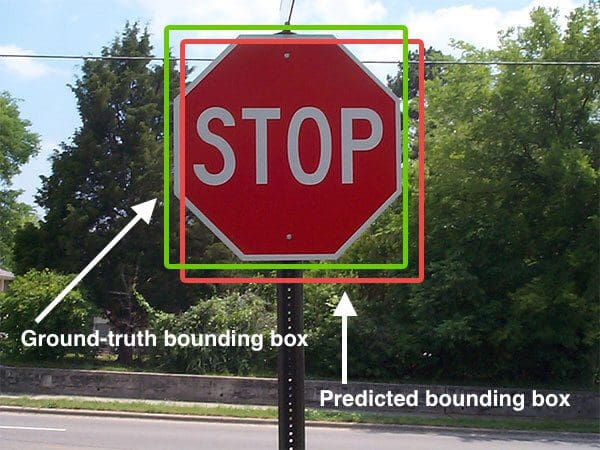
\includegraphics[scale=0.49]{pictures/iou_stop_sign.jpg}
            \caption{Die vorhergesagte Boundingbox wird in Rot dargestellt, während die Ground-Truth-Boundingbox in Grün dargestellt wird \cite{iou}.}
        \end{figure}

\newpage
        \cite{iou}
        Der IoU zwischen der vorhergesagten Boundingbox und der Ground-Truth-Boundingbox lässt sich einfach berechnen:
        Die Fläche der Schnittmenge wird durch die Fläche der Vereinigung der beiden Boundingboxen dividiert.
        
        \begin{center}  
            $Area = x2 y2 - x1 y1$\\
            wobei $x1y1$ obere linke Ecke und $x2y2$ untere rechte Ecke\\ \bigskip
            \large$IoU = \frac{Area_{Ground-Truth} \cap Area_{predicted}}{Area_{Ground-Truth} \cup Area_{predicted}}$
        \end{center}

        \begin{figure}[!htb]
            \centering
            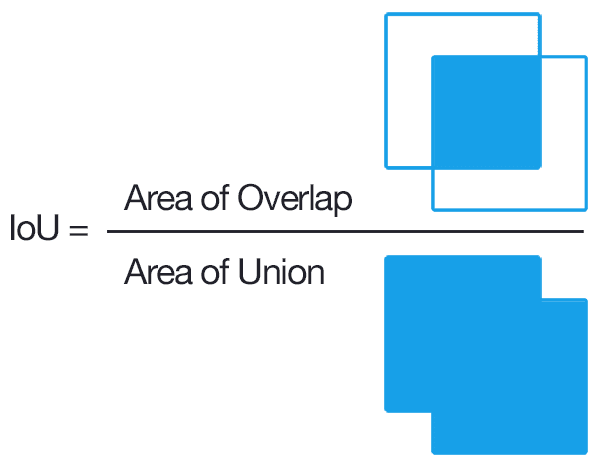
\includegraphics[scale=0.49]{pictures/iou_equation.png}
            \caption{Berechnung des IoU als Grafik \cite{iou}}.
        \end{figure}

        Bei der Verwendung von IoU als Bewertungsmetrik muss ein Schwellenwert (Threshold) für die Genauigkeit festgelegt werden, der in der Regel bei 0,5 liegt. Werte darüber werden als gut bewertet, während Werte darunter als unbrauchbar gelten \cite{iou_paper, iou_2}.
